\subsection{Actuator Morphologies}
\label{subsec:Actuators, Actuator Morphologies}
This section provides an in-depth look at three separate soft elastomer body segments actuated using pressurized fluids.
%
We use a defining structural feature to refer to each of the presented segment morphologies, those are (i) ribbed, (ii) cylindrical, and (iii) pleated.
%
In Section~\ref{sec:Manipulators}, these segments are combined serially to form multi-body manipulators and in Section~\ref{sec:Locomotion} they are used to form single and multi-body locomotory robots.
%
Although similar in material composition and function, differences in internal and external structure and form lead to several distinct difference between the three presented morphologies.
%
First, we present each morphology, examining the structural differences.
%
Then, we provide a comparative characterization of the segments, highlighting salient performance characteristics.

\subsubsection{Ribbed Segment}
\label{subsubsec:Actuators, Actuator Morphologies, Ribbed}
The ribbed fluidic elastomer actuator with its multiple rectangular channels was first implemented and characterized in \citet{correll2010soft} followed by \citet{onal2011soft, onal2013autonomous}.
%
Joining two fluidic elastomer actuators in an agonist-antagonist pairing provides bidirectional bending.
%
This actuator type provided the fundamental segment-level structure of the manipulator developed in \citet{marchese2014design}.
%
We refer to this three layer composite here as a ribbed segment.
%
That is, two actuator layers are combined in a pair, but separated by an inextensible constraint layer.
%
An implementation of this segment morphology is shown in both a neutral (Fig.~\ref{fig:ribbed design}A) and bent state (Fig.~\ref{fig:ribbed design}B).
%
Bending is produced through the pressurization of agonist fluidic channels (Fig.~\ref{fig:ribbed design}b) that are embedded within the actuated layers (Fig.~\ref{fig:ribbed design}, layers 1 and 3).
%
The structure of the actuated layers is cast from soft elastomer (Fig.~\ref{fig:ribbed design}a).
%
When pressurized, the agonist fluidic channels expand and strain the elastomer.
%
This deformation is transferred into bending by means of an inextensible but flexible constraint (Fig.~\ref{fig:ribbed design}c) embedded within the center layer (Fig.~\ref{fig:ribbed design}, layer 2).
%
Ribs located between channels (Fig.~\ref{fig:ribbed design}e) mitigate strain normal to the inextensible neutral axis.
%
At the segment level, \citet{marchese2014design} extended the ribbed segment design to make it suitable for inclusion in a multi-segment manipulator.
%
Specifically, fluidic supply channels (Fig.~\ref{fig:ribbed design}d) were introduced on either side of the inextensible constraint and embedded within the center layer.
%
Each segment accommodates multiple, parallel supply channels, two for each body segment within the manipulator.
%
For a detailed model of how a ribbed segment deforms under fluidic pressure input, please refer to \citet{marchese2014autonomous}. %why not adding it here?
%
It is important to note that this simplifying static model assumes that ribbed channels deform purely by extending their side and top walls, and that these wall stresses are based on initial channel geometry.
%
In reality, as is shown here in Algorithm~\ref{alg:SimpleModel}, wall stresses change as a function of the deformed geometry.
If needed, Algorithm \ref{alg:SimpleModel} can be used to augment the ribbed model in Chapter~\ref{chap:Single Segment Soft Robots}, Section~\ref{sec:Fish Actuation}.

\textbf{Pros}: The primary benefits of this morphology in relation to alternatives presented in this section are: (1) Ribs between channels mitigate strain normal to the neutral axis. (2) For a fixed fluid energy input, this segment exhibits greater bending than the cylindrical segment.

\textbf{Cons}: The primary disadvantages of this morphology in relation to alternatives presented in this section are: (1) The three layer structure is prone to delamination and rupture under high strain. (2) Manufacturing this rectangular, layered structure is challenging because all transmission lines must be embedded within the thin constraint layer.

\begin{figure}[htb]
\centering
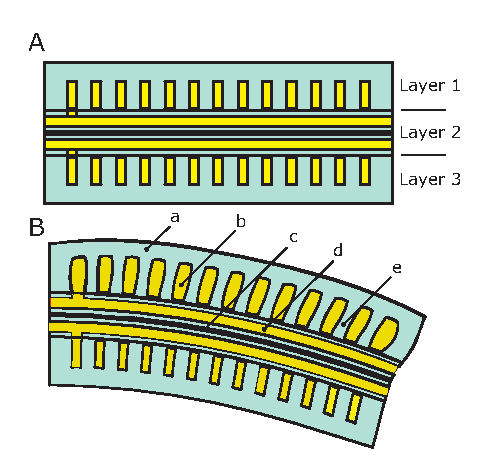
\includegraphics[width=2.9in]{Figures/actuators/ribbed_design.eps}
\caption[A conceptual representation of the ribbed segment morphology]{A conceptual representation of the ribbed segment morphology. The segment is composed of three layers produced from soft elastomer (a), embedded fluidic channels (b), inextensible, but flexible constraint (c), embedded fluid transmission lines (d), and ribbed structures (e). (\textbf{A}) The segment in an unactuated, or neutral state. (\textbf{B}) The segment in an actuated state where fluid within the agonist channel group is pressurized producing bending about the inextensible axis.} \label{fig:ribbed design}
\end{figure}

\subsubsection{Cylindrical Segment}
\label{subsubsec:Actuators, Actuator Morphologies, Cylindrical}
The cylindrical fluidic elastomer segment is an alternative to the ribbed design.
%
This design was first presented by the authors in \citet{marchese2014whole}.
%
Design inspiration was drawn from the soft rubber tentacles developed by \citet{martinez2013robotic} which use embedded crescent-shaped channels in a similar two-layer rubber construction.
%
Although the cylindrical segment morphology is notably different from the ribbed segment, the fundamental operating principles are the same.
%
In the cylindrical morphology (Fig.~\ref{fig:cylindrical_design}A and B), we transition from a rectangular, planar-layered composite to a cylindrical, concentric-layered composite.
%
Specifically, the segment consists of three concentric layers: (i) an outer soft layer (Fig.~\ref{fig:cylindrical_design}b, \emph{transparent}), (ii) a slightly stiffer inner layer (Fig.~\ref{fig:cylindrical_design}d, \emph{green}), and (iii) a hollow core that accommodates a bundle of fluid transmission lines (Fig.~\ref{fig:cylindrical_design}f, \emph{white}).
%
Two fluid-filled, and cylindrically-shaped channels are embedded laterally within the outermost layer (Fig.~\ref{fig:cylindrical_design}c).
%
These channels interface with the transmission lines by means of a stiffer rubber inlet piece (Fig.~\ref{fig:cylindrical_design}a, \emph{brown}).
%
When pressurized, the entrapped fluid deforms the embedded channel both circumferentially and longitudinally (Fig.~\ref{fig:cylindrical_design}B).
%
Specific to this morphology, the inner tube-like layer composed of slightly stiffer rubber serves as an inextensible constraint, transforming channel deformation into segment bending.

%%structural impendance two sentence

\textbf{Pros}: The primary benefits of this morphology in relation to alternatives presented in this section are: (1) Entirely composed of rubber, the resiliency and the durability of the actuator are increased. (2) The two cylindrical channels make this segment the simplest to fabricate. (3) Embedded fluidic channels are not at the interface between fabricated layers, making this morphology robust against delamination under high pressures.

\textbf{Cons}: The primary disadvantages of this morphology in relation to alternatives presented in this section are: (1) The simple channel design exhibits high circumferential strain. Compared to the ribbed and pleated morphologies, more fluid energy is required to produce bending. (2) When the segment bends, an increased volume of rubber on the antagonist side of the actuator has to be compressed. This inhibits a high maximum curvature.

\begin{figure}[htb]
\centering
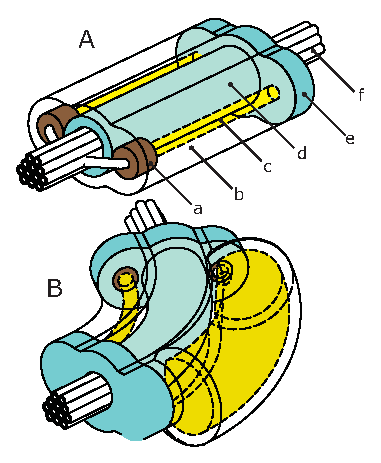
\includegraphics[width=2.9in]{Figures/actuators/cylindrical_design.eps}
\caption[A conceptual representation of the cylindrical segment morphology.]{A conceptual representation of the cylindrical segment morphology. The segment consists of a soft silicone rubber outer layer (b, \emph{transparent}), a slightly stiffer silicone inner layer (d, \emph{cyan}), crush resistant silicone inlets (a, brown), expanding embedded fluidic channels (c, \emph{yellow}), and an internal tubing bundle (f, \emph{white}). The segment terminates in soft endplates (e). (\textbf{A}) A depiction of the segment in an unactuated state. (\textbf{B}) A depiction of the body segment in an actuated state where the expansion of the pressurized fluidic channel is schematically represented.
}\label{fig:cylindrical_design}
\end{figure}

\subsubsection{Pleated Segment}
\label{subsubsec:Actuators, Actuator Morphologies, Pleated}
The pleated channel design is detailed in Figure~\ref{fig:pleated_design} and consists of evenly spaced, discrete elastomer sections (Fig.~\ref{fig:pleated_design}d), which are separated by gaps (Fig.~\ref{fig:pleated_design}c).
%
Embedded within each elastomer section is a hollow channel (Fig.~\ref{fig:pleated_design}e).
%
Cut views of the un-actuated and actuated states are shown in Figure~\ref{fig:pleated_design}A and Figure~\ref{fig:pleated_design}B, respectively.
%
This design approach draws inspiration for its pleats from the soft pneumatic gloves developed by \citet{polygerinos2013towards} and its homogeneous body design is inspired from the tail design of a soft robotic fish developed by \citet{katzschmann2014hydraulic}.
%
The hollow channels within each pleat are connected via a center channel and are accessible through a front inlet (Fig.~\ref{fig:pleated_design}a).
%
When fluid within these channels is pressurized (Fig.~\ref{fig:pleated_design}, \emph{yellow}), an individual pleat undergoes a balloon-like expansion of the thin exterior skin both normal and parallel to the neutral axis.
%
Similar to the cylindrical actuator design, a stiffer silicone layer (Fig.~\ref{fig:pleated_design}, \emph{blue}) serves as an almost inextensible constraint layer.
%
The sum of the balloon-like expanding motions leads to bending of the less extensible center constraint layer.

\textbf{Pros}: The primary benefits of this morphology in relation to alternatives presented in this section are: (1) A unidirectional pleated actuator is capable of bending to higher curvatures than the ribbed or cylindrical morphology.
(2) A bidirectional pleated segment is capable of exerting higher maximum forces because of its ability to accommodate the largest energy input.
(3) Using a lost-wax casting approach, the \emph{cyan} portion of this segment can be cured in a single step, avoiding seams that are prone to delamination.

\textbf{Cons}: The primary disadvantages of this morphology in relation to alternatives presented in this section are: (1) The morphology is more complex to manufacture because it requires a lost-wax casting procedure detailed in Section~\ref{subsubsec:PM Actuation, Fabrication, Pleated}. (2) The implementation of this morphology requires the most fluid energy to actuate it to appreciable tip forces. This might very well be due to the fact that, when compared to the other implementations, this implementation is larger in size and uses a higher shore hardness elastomer.

\begin{figure}[htb]
\centering
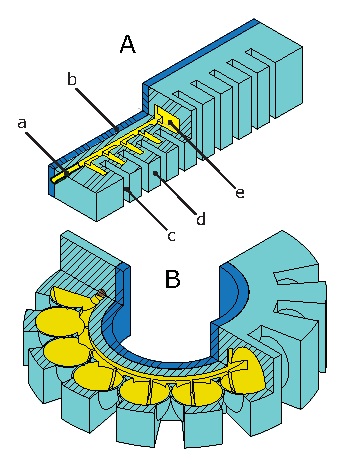
\includegraphics[width=2.9in]{figures/actuators/pleated_design.eps}
\caption[A conceptual representation of the pleated segment morphology.]{A conceptual representation of the pleated segment morphology. The design consists of a channel inlet (a), an almost inextensible constraint layer (b), uniform pleats (d) separated by even gaps (c), and internal channels within each pleat (e). (\textbf{A}) depicts the segment in an unactuated state and (\textbf{B}) shows the segment in an actuated and therefore bent state. The expansion of the pressurized channels are schematically represented.}\label{fig:pleated_design}
\end{figure}

\subsubsection{Comparative Characterization}
\label{subsubsec:Actuators, Actuator Morphologies, Characterization}
To characterize the actuated segments, we first perform bending tests to experimentally determine the relationship between the segment's neutral axis bend angle $\theta$, internal channel pressure $p_c$, and supplied volume $\mathbb{V}_s$ for each morphology.
%
In these experiments, the base of each segment is grounded securely in a fixture and the segment's tip is supported vertically with a ball transfer. %removed: ", if necessary." <-because this seems like vague statement
%
Then, the segment's agonist channel is incrementally filled under closed-loop volume control via the displacement of a fluidic drive cylinder; please refer to Section~\ref{sec:Power}.
%
After each incremental fill, we allow pressure within the cylinder and within the actuated channel to equalize before measurements of the channel's pressure and the segment's curvature are taken.
%
Curvature is assumed to be constant along the length of the segment and is uniquely defined by measuring the cartesian locations of the base and the tip of the segment; refer to \citet{marchese2014design}.
%
From this curvature we compute the segment's bend angle.
%
Since this is a quasi-static process, fluid pressure and supply volume measurements can be used to determine the elastic potential fluid energy input into the actuation system, which consists of the elastomer segment and the internal compressible transmission fluid.
The potential energy is calculated by
\begin{equation}\label{eqn:energy}
    V_{Elastic} = \int_0^{\mathbb{V}_c} p_c\left( \mathbb{V} \right) \, \text{d} \mathbb{V}.
\end{equation}
%
Additionally, a blocking force test is performed in order to understand the variability in tip force output between segment morphologies.
%
Again, a similar experimental procedure is used as for the bending characterization; however, during blocking force experiments a plate attached via a force transducer to ground is mounted in contact with the segment's tip, orthogonal to the bending plane.
%
This effectively measures the force required to block the actuator from bending.
%
\begin{figure*}[htb]
        \centering
        \begin{subfigure}[b]{0.95\columnwidth}
            \centering
            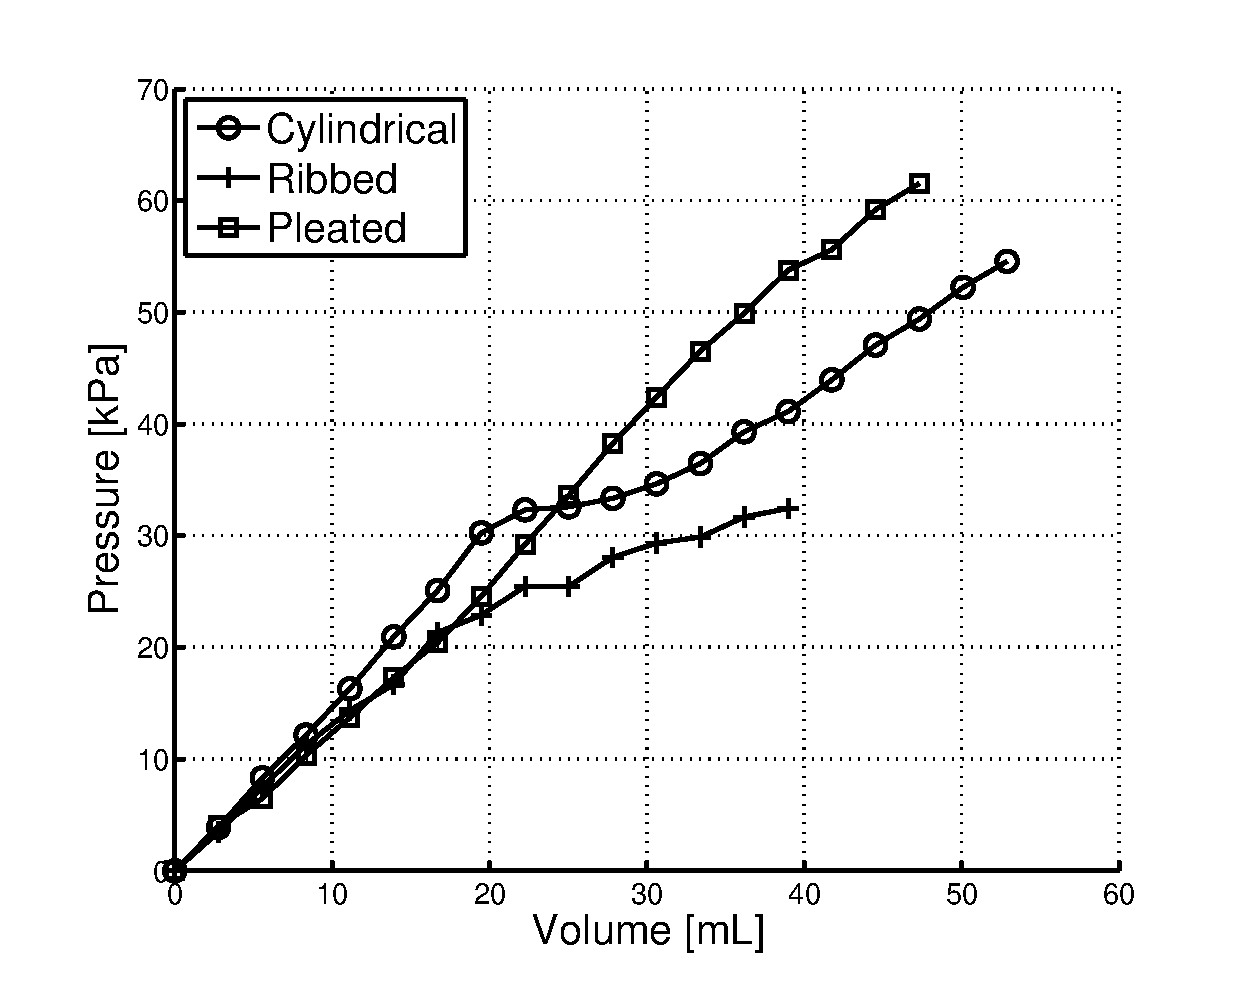
\includegraphics[width=0.95\columnwidth]{figures/actuators/morphologiescharacterization/PressureVsVolume.eps}
            \caption{}
            \label{fig:Characterization_PressureVsVolume}
        \end{subfigure}
        \begin{subfigure}[b]{0.95\columnwidth}
            \centering
            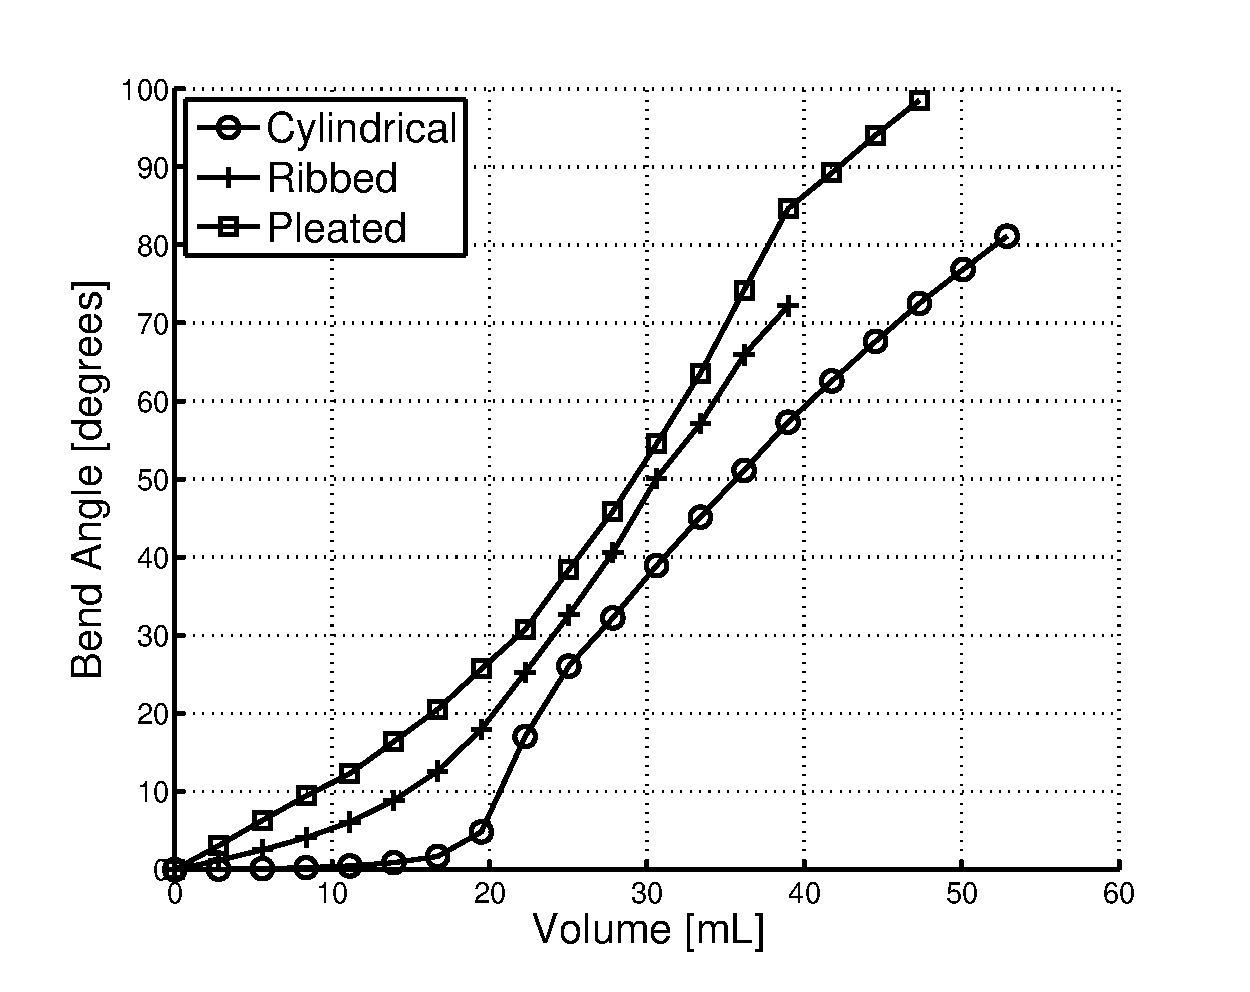
\includegraphics[width=0.95\columnwidth]{figures/actuators/morphologiescharacterization/BendAngleVsVolume.eps}
            \caption{}
            \label{fig:Characterization_CurvatureVsVolume}
        \end{subfigure} \\
        \begin{subfigure}[b]{0.95\columnwidth}
            \centering
            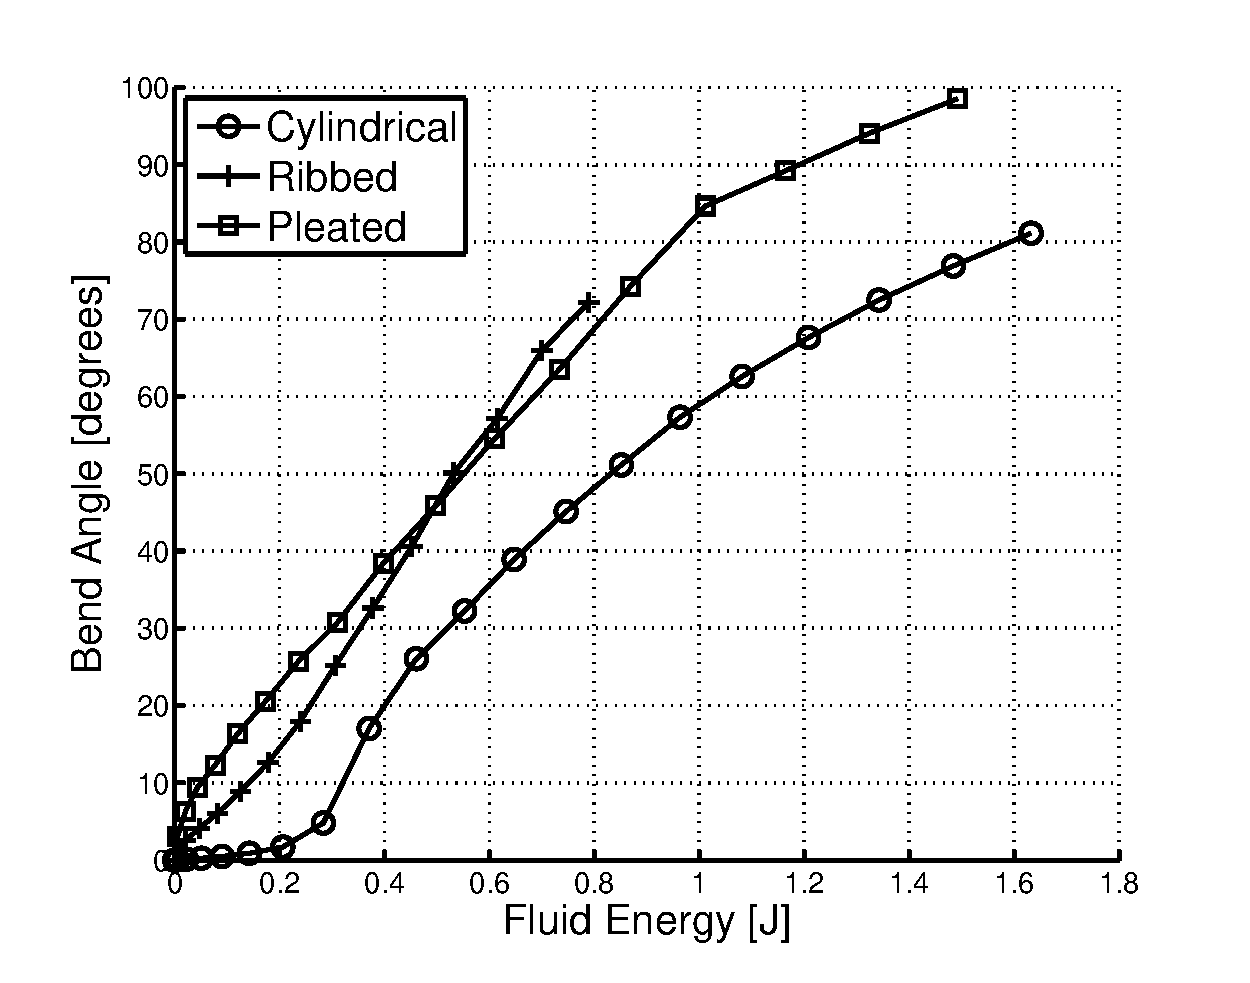
\includegraphics[width=0.95\columnwidth]{figures/actuators/morphologiescharacterization/BendAngleVsEnergy.eps}
            \caption{}
            \label{fig:Characterization_CurvatureVsEnergy}
        \end{subfigure}
        \begin{subfigure}[b]{0.95\columnwidth}
            \centering
            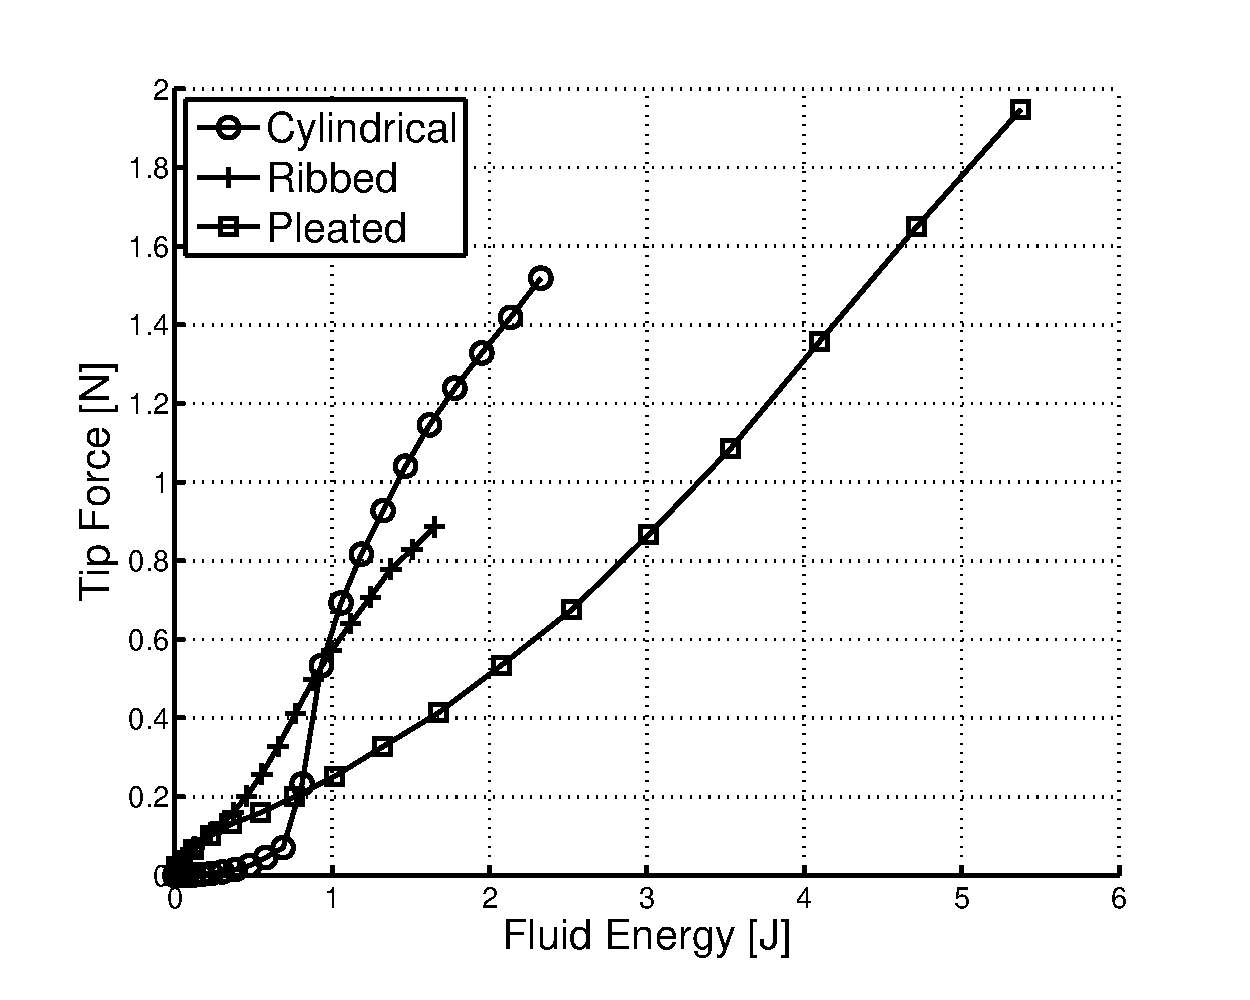
\includegraphics[width=0.95\columnwidth]{figures/actuators/morphologiescharacterization/ForceVsEnergy.eps}
            \caption{}
            \label{fig:Characterization_ForceVsEnergy}
        \end{subfigure}
        \caption[Experimental characterizations of three actuated segment morphologies.]{Experimental characterizations of three actuated segment morphologies performed by filling each actuator by means of controlled volumetric displacements and measuring internal pressure, neutral axis bend angle under a constant-curvature assumption, and blocking force.}\label{fig:actuator_characterization}
\end{figure*}

Figure~\ref{fig:actuator_characterization} details the results of these characterization experiments from which we can make several observations.
%
First, the pleated morphology is generally the stiffest, followed by the cylindrical, and then the ribbed, where stiffness is defined as $\frac{\partial p_c}{\partial \mathbb{V}_c}$ (Fig.~\ref{fig:Characterization_PressureVsVolume}).
%
Second, the cylindrical morphology has a salient bend angle nonlinearity (Fig.~\ref{fig:Characterization_CurvatureVsVolume}).
%
More specifically, small volumetric fluid changes of less than $15\,$mL provide little control authority over curvature; however, above $25\,$mL displacements, the control authority is strong and the curvature-volume relationship is approximately linear.
%
Third, the cylindrical morphology requires the most amount of fluid energy to produce a given bend angle and the ribbed and pleated segments require approximately the same amount of fluid energy to generate equivalent bending (Fig.~\ref{fig:Characterization_CurvatureVsEnergy}).
%
Lastly, the pleated segment generally requires more fluid energy than both the ribbed and cylindrical morphologies to produce a given tip force.
%
However, the pleated segment can accommodate significantly higher input energies and therefore can reach the highest maximum tip force. 